% =============================================================================
%  MATE 6026 -- Optimización Numérica -- Proyecto Final
%  Universidad de Puerto Rico, Recinto de Mayagüez
%  Compile with: pdflatex -> bibtex -> pdflatex -> pdflatex
% =============================================================================
\documentclass[11pt,letterpaper]{article}
 
% --- Geometry and spacing --------------------------------------------------
\usepackage[margin=1in]{geometry}
\usepackage{setspace}
\onehalfspacing
 
% --- Encoding and fonts ----------------------------------------------------
\usepackage[utf8]{inputenc}
\usepackage[T1]{fontenc}
\usepackage{lmodern}
\usepackage{microtype}
 
% --- Math ------------------------------------------------------------------
\usepackage{amsmath,amssymb,amsthm,mathtools}
\usepackage{bm}
 
% --- Graphics and floats ---------------------------------------------------
\usepackage{graphicx}
\usepackage{booktabs}
\usepackage{caption}
\usepackage{subcaption}
\usepackage{float}
 
% --- Algorithms ------------------------------------------------------------
\usepackage{algorithm}
\usepackage{algpseudocode}
 
% --- Tables and arrays -----------------------------------------------------
\usepackage{array}
\usepackage{multirow}
 
% --- References and links --------------------------------------------------
\usepackage[numbers,sort&compress]{natbib}
\usepackage[hidelinks]{hyperref}
\usepackage{cleveref}
 
% --- Custom commands -------------------------------------------------------
\newcommand{\R}{\mathbb{R}}
\newcommand{\N}{\mathbb{N}}
\newcommand{\E}{\mathbb{E}}
\newcommand{\norm}[1]{\left\|#1\right\|}
\newcommand{\inner}[2]{\left\langle #1, #2 \right\rangle}
\newcommand{\T}{^{\mathsf{T}}}
\newcommand{\grad}{\nabla}
\DeclareMathOperator*{\argmin}{arg\,min}
\DeclareMathOperator{\RMSE}{RMSE}
\DeclareMathOperator{\MSE}{MSE}
 
% --- Theorem-like environments --------------------------------------------
\theoremstyle{definition}
\newtheorem{definition}{Definition}[section]
\newtheorem{assumption}{Assumption}[section]
\newtheorem{remark}{Remark}[section]
 
% --- Title information -----------------------------------------------------
\title{%
  \Large
  First- and Second-Order Optimization Methods for\\
  Neural Network Regression:\\
  A Comparative Study of Levenberg--Marquardt,\\
  Nonlinear Conjugate Gradient, and Adam
}
 
\author{%
  Author One\thanks{Department of Mathematical Sciences, University of Puerto Rico at Mayagüez. Correspondence: \texttt{author.one@upr.edu}.} \and
  Author Two\footnotemark[1] \and
  Author Three\footnotemark[1]
}
 
\date{MATE 6026 --- Numerical Optimization \\ Final Project Report \\ \today}
 
% =============================================================================
\begin{document}
% =============================================================================
 
\maketitle
 
\begin{abstract}
\noindent
Training a feedforward neural network with mean-squared-error loss is, in formal
terms, a nonlinear least squares problem in the network parameters. This
correspondence places the problem within the scope of classical numerical
optimization and invites a direct comparison between methods designed for
that setting and the stochastic first-order methods favored in modern practice.
We compare three optimizers on a tabular regression benchmark: the
Levenberg--Marquardt method (LM), which exploits the Gauss--Newton Hessian
approximation; the nonlinear conjugate gradient method (NCG) with
Polak--Ribière\textsuperscript{+} updates and a strong Wolfe line search; and
Adam, representative of contemporary adaptive stochastic methods. All three
are implemented in MATLAB over a shared infrastructure and compared on the
UCI Concrete Compressive Strength dataset across five random seeds. We report
convergence per iteration, wall-clock efficiency, and test-set generalization.
The results are interpreted in the light of the theoretical properties
developed in Chapters 3, 5, and 10 of \citet{NocedalWright2006}.
\end{abstract}
 
\bigskip
\noindent
\textbf{Keywords:} nonlinear least squares; Levenberg--Marquardt; nonlinear
conjugate gradient; Adam; neural network regression; numerical optimization.
 
\vspace{1em}
\hrule
 
% =============================================================================
\section{Introduction}
\label{sec:introduction}
% =============================================================================
 
\subsection{Motivation}
 
Neural networks are now the default modeling tool for a broad range of
supervised learning problems, and their training is almost universally
carried out by stochastic first-order methods with adaptive step sizes, of
which Adam~\citep{KingmaBa2015} is the most widely used. This uniformity of
practice tends to obscure a basic structural question that sits squarely
within the scope of numerical optimization: \emph{how does the training of a
neural network relate to the classical problems treated in a graduate
optimization course, and do the methods designed for those problems remain
competitive?}
 
For regression tasks under the mean squared error loss, the connection is
exact rather than analogical. Training a network $f(\,\cdot\,;\theta)$ on
data $\{(x_i, y_i)\}_{i=1}^N$ to minimize
\begin{equation}
L(\theta)
\;=\; \tfrac{1}{2}\sum_{i=1}^{N}\bigl(y_i - f(x_i;\theta)\bigr)^{2}
\label{eq:loss-intro}
\end{equation}
is a \emph{nonlinear least squares} problem in $\theta$, and hence the subject
of Chapter~10 of~\citet{NocedalWright2006}. This observation suggests that
methods designed to exploit the sum-of-squares structure --- the
Gauss--Newton method and its regularized variant, the Levenberg--Marquardt
algorithm --- may apply directly. It also permits a well-posed comparison
against first-order methods (Chapter~5) and against the adaptive
stochastic baseline that dominates current practice.
 
\subsection{Problem studied}
 
We compare three optimization algorithms applied to the same neural network
regression problem:
\begin{itemize}
  \item \textbf{Levenberg--Marquardt (LM)}: a trust-region-like method for
    nonlinear least squares that interpolates between Gauss--Newton and
    scaled steepest descent by means of an adaptive damping parameter
    \citep[Ch.~10]{NocedalWright2006}.
  \item \textbf{Nonlinear Conjugate Gradient (NCG)}: a first-order method
    with Polak--Ribière\textsuperscript{+} updates and a strong Wolfe line
    search \citep[Ch.~5]{NocedalWright2006}.
  \item \textbf{Adam}: an adaptive stochastic first-order method
    \citep{KingmaBa2015}, serving as the state-of-the-art baseline.
\end{itemize}
The three methods span a clean spectrum of information usage. LM employs
the Gauss--Newton Hessian approximation $J\T J$; NCG uses only gradients and
a single previous search direction; Adam uses gradients together with
diagonal second-moment estimates. The comparison is therefore less a
benchmark race than a controlled study of \emph{how much curvature
information is useful for this class of problems, and at what computational
cost}.
 
\subsection{Context in the literature}
 
The application of Levenberg--Marquardt to neural network training is not
new. \citet{HaganMenhaj1994} showed that LM substantially outperforms
backpropagation with momentum on small-to-medium fully connected networks,
and the method remains available in MATLAB's Neural Network Toolbox for
this reason. Nonlinear conjugate gradient methods were standard for
network training prior to the widespread adoption of stochastic methods
\citep{Moller1993}. Adam emerged in the deep learning era
\citep{KingmaBa2015} and has since become the de facto default.
 
Despite this history, direct empirical comparisons across these three
method families on a common problem, with controlled initialization and
matched stopping criteria, are surprisingly rare in the pedagogical
literature. We target the intermediate regime --- a few hundred parameters,
roughly a thousand training examples --- in which all three methods are
tractable and competitive.
 
\subsection{Scope}
 
The study is deliberately narrow. We restrict attention to (i) regression
problems, in which the nonlinear least squares framing applies; (ii)
tabular data, which permits parameter counts small enough for LM to be
practical; (iii) a single fully connected architecture, to isolate optimizer
behavior from architectural choices; and (iv) serial CPU execution, for
interpretable wall-clock measurements. Each of these choices is revisited
in the discussion.
 
\subsection{Contributions and organization}
 
Our contributions are threefold: (a) a unified derivation of the three
methods in a common notation, anchored in the nonlinear least squares
formulation; (b) a controlled empirical comparison on a standard regression
benchmark, with five-seed statistics for every reported quantity; and (c)
a regime analysis relating the observed behavior to the theoretical
properties developed in class.
 
The remainder of the report is organized as follows.
\Cref{sec:objectives} states the objectives.
\Cref{sec:problem} formulates the problem and derives the three methods in
a common framework.
\Cref{sec:methodology} describes the experimental protocol.
\Cref{sec:results} presents the numerical results.
\Cref{sec:conclusions} concludes and discusses limitations.
 
% =============================================================================
\section{Objectives}
\label{sec:objectives}
% =============================================================================
 
\paragraph{General objective.}
To compare three optimization methods --- Levenberg--Marquardt, Nonlinear
Conjugate Gradient, and Adam --- for training a feedforward neural network
on a tabular regression task, framed as a nonlinear least squares problem.
 
\paragraph{Specific objectives.}
\begin{enumerate}
  \item Formulate neural network regression under MSE loss as a nonlinear
    least squares problem and derive the gradient and Gauss--Newton Hessian
    approximation in terms of the residual Jacobian $J(\theta)$.
  \item Implement LM, NCG with strong Wolfe line search, and Adam in
    MATLAB, built on a shared infrastructure for residual evaluation,
    Jacobian computation, and logging.
  \item Evaluate each optimizer along three axes --- convergence per
    iteration, wall-clock efficiency, and test-set RMSE --- on the UCI
    Concrete Compressive Strength dataset.
  \item Characterize the regimes in which each method is preferable,
    relating empirical behavior to the theoretical properties discussed in
    \citet[Chs.~3, 5, 10]{NocedalWright2006}.
  \item Assess sensitivity to initialization and hyperparameters through
    repeated trials over five independent random seeds.
\end{enumerate}
 
% =============================================================================
\section{Problem formulation}
\label{sec:problem}
% =============================================================================
 
\subsection{Regression setup}
 
Let $\mathcal{D} = \{(x_i, y_i)\}_{i=1}^{N}$ be a dataset of
input--output pairs with $x_i \in \R^{d}$ and $y_i \in \R$. We assume a
data-generating relation
\begin{equation}
y_i = \varphi(x_i) + \varepsilon_i, \qquad
\varepsilon_i \overset{\text{iid}}{\sim} \mathcal{N}(0, \sigma^2),
\label{eq:data-gen}
\end{equation}
for some unknown $\varphi : \R^d \to \R$, and seek to approximate $\varphi$
by a parametric model $f(\,\cdot\,;\theta)$ with parameter vector
$\theta \in \R^{n}$.
 
\subsection{Neural network parametrization}
 
The model $f(\,\cdot\,;\theta)$ is a fully connected feedforward network
with $L$ layers. Given weights
$W^{(\ell)} \in \R^{n_\ell \times n_{\ell-1}}$ and biases
$b^{(\ell)} \in \R^{n_\ell}$ for $\ell = 1,\ldots,L$, the forward pass is
\begin{equation}
a^{(0)} = x,\qquad
z^{(\ell)} = W^{(\ell)} a^{(\ell-1)} + b^{(\ell)},\qquad
a^{(\ell)} = \sigma\bigl(z^{(\ell)}\bigr),
\label{eq:forward}
\end{equation}
for $\ell = 1,\ldots,L-1$, where $\sigma(\cdot) = \tanh(\cdot)$ is applied
componentwise. The output layer is linear:
\begin{equation}
f(x;\theta) = W^{(L)} a^{(L-1)} + b^{(L)}.
\label{eq:output}
\end{equation}
The parameter vector $\theta \in \R^n$ stacks all entries of
$\{W^{(\ell)}, b^{(\ell)}\}_{\ell=1}^{L}$, with
\begin{equation}
n \;=\; \sum_{\ell=1}^{L}\bigl(n_\ell\, n_{\ell-1} + n_\ell\bigr).
\end{equation}
For the architecture $d \to 16 \to 16 \to 1$ with $d = 8$, this gives
$n = 433$ trainable parameters.
 
\subsection{Nonlinear least squares formulation}
 
Define the residual of the $i$-th example,
\begin{equation}
r_i(\theta) = y_i - f(x_i;\theta), \qquad i = 1,\ldots, N,
\label{eq:residual-def}
\end{equation}
and collect the residuals in the vector
$r(\theta) = \bigl(r_1(\theta),\ldots, r_N(\theta)\bigr)\T \in \R^{N}$.
The training problem is the nonlinear least squares problem
\begin{equation}
\boxed{\;
\min_{\theta \in \R^{n}}\;
L(\theta)
\;:=\;
\tfrac{1}{2}\,\norm{r(\theta)}_2^{2}
\;=\;
\tfrac{1}{2}\sum_{i=1}^{N} r_i(\theta)^{2}.
\;}
\label{eq:nls}
\end{equation}
The objective $L : \R^n \to \R$ is continuously differentiable but
\emph{not convex} in $\theta$, as the composition of affine maps with
$\tanh$ activations produces multiple critical points related by sign
and permutation symmetries \citep[see, e.g.,][]{Goodfellow2016}. We
therefore seek a local minimizer.
 
\subsection{Gradient and Jacobian}
 
The gradient of $L$ admits the compact form
\begin{equation}
\grad L(\theta) \;=\; J(\theta)\T\, r(\theta),
\label{eq:gradient}
\end{equation}
where $J(\theta) \in \R^{N \times n}$ is the Jacobian of the residual,
whose $i$-th row is
\begin{equation}
\bigl[J(\theta)\bigr]_{i,:}
\;=\;
\grad_\theta\, r_i(\theta)\T
\;=\;
-\grad_\theta\, f(x_i; \theta)\T.
\label{eq:jacobian-row}
\end{equation}
The exact Hessian decomposes as
\begin{equation}
\grad^{2} L(\theta)
\;=\;
J(\theta)\T J(\theta)
\;+\;
\sum_{i=1}^{N} r_i(\theta)\, \grad^{2} r_i(\theta).
\label{eq:hessian-decomp}
\end{equation}
When the residuals $r_i$ are small or the $\grad^2 r_i$ are bounded, the
first term dominates and the Gauss--Newton approximation
\begin{equation}
\grad^{2} L(\theta) \;\approx\; J(\theta)\T J(\theta)
\label{eq:gauss-newton}
\end{equation}
is justified. This is the structural fact on which LM rests.
 
\subsection{The three methods}
\label{sec:methods}
 
Each method generates iterates $\{\theta_k\}_{k \geq 0}$ via
$\theta_{k+1} = \theta_k + \alpha_k p_k$, differing in how the search
direction $p_k$ and step length $\alpha_k$ are chosen.
 
\subsubsection{Levenberg--Marquardt}
\label{sec:lm}
 
The LM search direction solves the regularized normal equations
\begin{equation}
\bigl(J_k\T J_k + \lambda_k I\bigr)\, p_k
\;=\; -J_k\T r_k,
\label{eq:lm-step}
\end{equation}
where $J_k = J(\theta_k)$, $r_k = r(\theta_k)$, and $\lambda_k \geq 0$ is
the damping parameter. The step is taken as $\alpha_k = 1$ and accepted
or rejected based on the gain ratio
\begin{equation}
\rho_k
\;=\;
\frac{L(\theta_k) - L(\theta_k + p_k)}{L(\theta_k) - m_k(p_k)},
\qquad
m_k(p) \;=\; \tfrac{1}{2}\,\norm{r_k + J_k p}_2^{2}.
\label{eq:gain-ratio}
\end{equation}
If $\rho_k$ is sufficiently large the step is accepted and $\lambda_k$ is
decreased (trusting the Gauss--Newton direction more); otherwise the step
is rejected and $\lambda_k$ is increased (falling back toward scaled
steepest descent). Pseudocode is given in
\cref{alg:lm}.
 
\begin{algorithm}[H]
\caption{Levenberg--Marquardt for nonlinear least squares}
\label{alg:lm}
\begin{algorithmic}[1]
\Require Initial $\theta_0$, $\lambda_0 > 0$, scaling factor $\nu > 1$,
  tolerances
\State $k \gets 0$
\Repeat
  \State Compute $r_k = r(\theta_k)$ and $J_k = J(\theta_k)$
  \State Solve $\bigl(J_k\T J_k + \lambda_k I\bigr)\, p_k = -J_k\T r_k$
  \State Compute gain ratio $\rho_k$ via~\cref{eq:gain-ratio}
  \If{$\rho_k > \rho_{\text{accept}}$}
    \State $\theta_{k+1} \gets \theta_k + p_k$
    \State $\lambda_{k+1} \gets \lambda_k / \nu$
  \Else
    \State $\theta_{k+1} \gets \theta_k$
    \State $\lambda_{k+1} \gets \lambda_k \cdot \nu$
  \EndIf
  \State $k \gets k+1$
\Until{$\norm{\grad L(\theta_k)}_\infty < \varepsilon$ or $k \geq k_{\max}$}
\end{algorithmic}
\end{algorithm}
 
\subsubsection{Nonlinear Conjugate Gradient (Polak--Ribière\textsuperscript{+})}
\label{sec:ncg}
 
Let $g_k = \grad L(\theta_k)$. The NCG direction is built recursively:
\begin{equation}
p_0 = -g_0, \qquad
p_{k+1} = -g_{k+1} + \beta_{k+1}^{\mathrm{PR+}}\, p_k,
\label{eq:ncg-direction}
\end{equation}
with the Polak--Ribière\textsuperscript{+} coefficient
\begin{equation}
\beta_{k+1}^{\mathrm{PR+}}
\;=\;
\max\!\left\{
\frac{g_{k+1}\T\,(g_{k+1} - g_k)}{g_k\T g_k},\;
0
\right\}.
\label{eq:pr-plus}
\end{equation}
The step length $\alpha_k$ is chosen to satisfy the strong Wolfe
conditions \citep[Algorithms~3.5--3.6]{NocedalWright2006}:
\begin{align}
L(\theta_k + \alpha_k p_k) &\leq L(\theta_k) + c_1\, \alpha_k\, g_k\T p_k,
\label{eq:wolfe-1}\\[2pt]
\bigl|\grad L(\theta_k + \alpha_k p_k)\T p_k\bigr|
  &\leq c_2\, \bigl|g_k\T p_k\bigr|,
\label{eq:wolfe-2}
\end{align}
with $c_1 = 10^{-4}$ and $c_2 = 0.1$. A restart
$p_k \leftarrow -g_k$ is triggered every $n$ iterations or whenever
$\beta^{\mathrm{PR+}} = 0$.
 
\subsubsection{Adam}
\label{sec:adam}
 
Given a mini-batch $\mathcal{B}_k \subset \{1,\ldots, N\}$ and the
stochastic gradient
$\tilde g_k = \grad L_{\mathcal{B}_k}(\theta_k)$, Adam maintains
exponential moving averages of the first two moments:
\begin{align}
m_k &= \beta_1 m_{k-1} + (1 - \beta_1)\, \tilde g_k, \\
v_k &= \beta_2 v_{k-1} + (1 - \beta_2)\, \tilde g_k \odot \tilde g_k,
\end{align}
with bias-corrected estimates
$\hat m_k = m_k/(1-\beta_1^{k})$ and
$\hat v_k = v_k/(1-\beta_2^{k})$, and update
\begin{equation}
\theta_{k+1}
\;=\;
\theta_k - \alpha\, \hat m_k \oslash \bigl(\sqrt{\hat v_k} + \epsilon\bigr),
\label{eq:adam-update}
\end{equation}
where $\odot$ and $\oslash$ denote componentwise product and division, and
$\beta_1 = 0.9$, $\beta_2 = 0.999$, $\epsilon = 10^{-8}$ are the default
hyperparameters of \citet{KingmaBa2015}.
 
\begin{remark}
\label{rem:batch-asymmetry}
LM and NCG are full-batch methods: both \cref{eq:lm-step} and
\cref{eq:ncg-direction} require the full gradient or Jacobian. Adam is used
in its standard mini-batch form. This asymmetry is genuine and is
revisited in the discussion~(\cref{sec:conclusions}).
\end{remark}
 
% =============================================================================
\section{Experimental methodology}
\label{sec:methodology}
% =============================================================================
 
\subsection{Dataset}
 
We use the UCI Concrete Compressive Strength
dataset~\citep{Yeh1998,UCIML}, comprising $N = 1{,}030$ samples with
$d = 8$ input features (cement, blast furnace slag, fly ash, water,
superplasticizer, coarse aggregate, fine aggregate, and age) and a single
target (compressive strength in MPa). The data are partitioned into
$70\%/15\%/15\%$ training/validation/test splits, stratified by target
quantile. Features and target are standardized to zero mean and unit
variance using training-set statistics only; all reported RMSE values are
converted back to the original MPa units for interpretability.
 
\subsection{Architecture and initialization}
 
We use a fully connected network $8 \to 16 \to 16 \to 1$ with
$\tanh$ activations and linear output, for a total of $n = 305$ parameters.
Weights are initialized by Glorot (Xavier) uniform sampling and biases are
initialized to zero \citep{GlorotBengio2010}. Within each seed, the same
initial $\theta_0$ is used for all three optimizers to isolate
optimizer-driven differences.
 
\subsection{Hyperparameters and stopping criteria}
 
Hyperparameters are summarized in \cref{tab:hyperparameters}. LM and NCG
terminate at $\norm{\grad L(\theta_k)}_\infty < 10^{-5}$ or after $500$
iterations. Adam runs for up to $2{,}000$ epochs with early stopping on
validation loss (patience $50$).
 
\begin{table}[H]
\centering
\small
\caption{Hyperparameter configuration.}
\label{tab:hyperparameters}
\begin{tabular}{@{}lll@{}}
\toprule
Method & Parameter & Value \\
\midrule
LM  & Initial damping $\lambda_0$            & $10^{-3}$ \\
LM  & Damping update factor $\nu$            & $10$ \\
LM  & Acceptance threshold $\rho_{\text{accept}}$ & $10^{-4}$ \\
\addlinespace
NCG & Wolfe constants $(c_1, c_2)$           & $(10^{-4},\, 0.1)$ \\
NCG & Restart period                         & $n$ iterations \\
\addlinespace
Adam & Learning rate $\alpha$                & Tuned on validation \\
Adam & Moment decays $(\beta_1, \beta_2)$    & $(0.9,\, 0.999)$ \\
Adam & Numerical stability $\epsilon$        & $10^{-8}$ \\
Adam & Mini-batch size                       & $32$ \\
\addlinespace
Common & Gradient tolerance $\varepsilon$    & $10^{-5}$ \\
Common & Max iterations / epochs             & $500\,/\,2000$ \\
Common & Random seeds                        & $\{0,1,2,3,4\}$ \\
\bottomrule
\end{tabular}
\end{table}
 
Adam's learning rate is selected on the validation set over the grid
$\{10^{-4}, 3\!\times\!10^{-4}, 10^{-3}, 3\!\times\!10^{-3}, 10^{-2}\}$.
LM and NCG use the textbook defaults above without additional tuning.
 
\subsection{Metrics}
 
For each run we log, at every iteration, the training loss
$L(\theta_k)$, the gradient norm $\norm{\grad L(\theta_k)}_\infty$,
the validation loss, and the cumulative wall-clock time. The final
parameters $\theta^\star$ produced by each method are evaluated on the
held-out test set using
\begin{equation}
\RMSE_{\text{test}}(\theta)
\;=\;
\sqrt{\frac{1}{|\mathcal{T}|}\sum_{i \in \mathcal{T}}
\bigl(y_i - f(x_i;\theta)\bigr)^{2}},
\label{eq:rmse}
\end{equation}
reported in MPa after inverting the target standardization.
 
\subsection{Implementation}
 
All code is written in MATLAB \texttt{[VERSION]}, executed
single-threaded on \texttt{[CPU MODEL]} with \texttt{[RAM]}. The residual
Jacobian $J(\theta)$ is computed by an analytical backpropagation routine
and cross-checked against centered finite differences at random $\theta$
values to a relative tolerance of $10^{-6}$. LM solves~\cref{eq:lm-step}
via MATLAB's \texttt{mldivide} operator. NCG and Adam are implemented
from scratch. All wall-clock measurements exclude data loading and
preprocessing.
 
% =============================================================================
\section{Results}
\label{sec:results}
% =============================================================================
 
\begin{remark}[Template note]
The numerical values in this section are placeholders, to be replaced by
the outputs of the experiments described in~\cref{sec:methodology}. The
structure of plots and tables is fixed in advance to ensure a fair
comparison across methods.
\end{remark}
 
\subsection{Convergence per iteration}
\label{sec:res-convergence}
 
\Cref{fig:loss-vs-iter} shows training loss versus iteration
(or epoch, for Adam) on a logarithmic scale, averaged over five seeds with
$\pm 1$ standard deviation bands. \Cref{tab:iters-to-tol} reports the
number of iterations required to reach training loss below
$\tau_L = \texttt{[THRESHOLD]}$.
 
\begin{figure}[H]
\centering
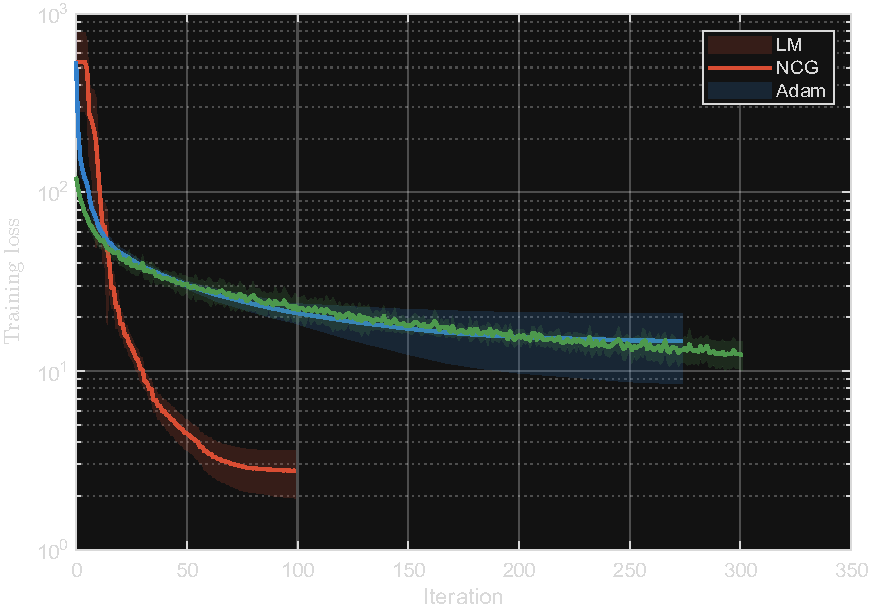
\includegraphics[width=0.85\linewidth]{figures/loss_vs_iter.pdf}
\caption{Training loss $L(\theta_k)$ vs.\ iteration $k$, log scale, three
curves (LM, NCG, Adam), mean $\pm 1$ std over five seeds.}
\label{fig:loss-vs-iter}
\end{figure}
 
\begin{table}[H]
\centering
\small
\caption{Iterations (or epochs for Adam) required to reach training loss
$L(\theta_k) \leq \tau_L$. Mean $\pm$ std over five seeds;
``DNC'' indicates methods that did not converge within the iteration
budget.}
\label{tab:iters-to-tol}
\begin{tabular}{@{}lrr@{}}
\toprule
Method & Iterations to $\tau_L$ & Seeds converged \\
\midrule
LM   & \texttt{[X $\pm$ X]} & \texttt{[X/5]} \\
NCG  & \texttt{[X $\pm$ X]} & \texttt{[X/5]} \\
Adam & \texttt{[X $\pm$ X]} & \texttt{[X/5]} \\
\bottomrule
\end{tabular}
\end{table}
 
\subsection{Wall-clock efficiency}
\label{sec:res-walltime}
 
\Cref{fig:loss-vs-time} shows training loss versus cumulative wall-clock
time on log--log axes. \Cref{tab:time-to-tol} reports wall-clock seconds
to the same tolerance $\tau_L$ used in \cref{tab:iters-to-tol}.
 
\begin{figure}[H]
\centering
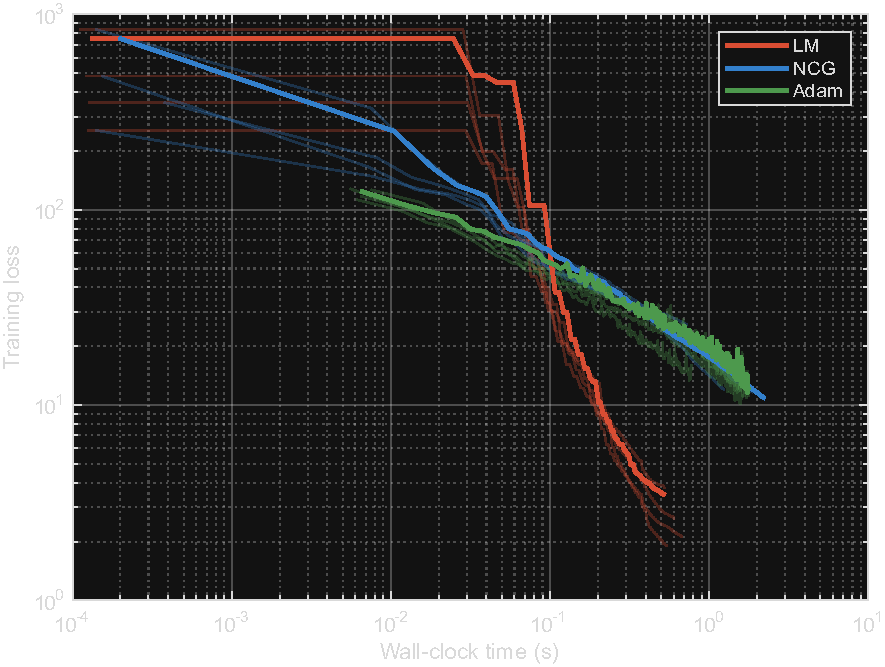
\includegraphics[width=0.85\linewidth]{figures/loss_vs_time.pdf}
\caption{Training loss vs.\ cumulative wall-clock time (log--log). Thin
traces: each seed individually. Thick traces: seed 0 highlighted for
each method.}
\label{fig:loss-vs-time}
\end{figure}
 
\begin{table}[H]
\centering
\small
\caption{Wall-clock time (seconds) to reach training loss
$L(\theta_k) \leq \tau_L$. Mean $\pm$ std over five seeds.}
\label{tab:time-to-tol}
\begin{tabular}{@{}lr@{}}
\toprule
Method & Time to $\tau_L$ (s) \\
\midrule
LM   & \texttt{[X $\pm$ X]} \\
NCG  & \texttt{[X $\pm$ X]} \\
Adam & \texttt{[X $\pm$ X]} \\
\bottomrule
\end{tabular}
\end{table}
 
\subsection{Generalization}
\label{sec:res-generalization}
 
\Cref{tab:test-rmse} is the primary quantitative summary: train,
validation, and test RMSE for each method, with total training time,
averaged over five seeds. Values are in MPa after inverting the target
standardization. \Cref{fig:pred-vs-actual} shows test-set predictions
versus actual values with $y = x$ overlaid.
 
\begin{table}[H]
\centering
\small
\caption{Final RMSE (MPa) and training time for each method, mean $\pm$ std
over five seeds. Lower is better for RMSE.}
\label{tab:test-rmse}
\begin{tabular}{@{}lrrrr@{}}
\toprule
Method & Train RMSE & Val RMSE & Test RMSE & Train time (s) \\
\midrule
LM   & \texttt{[X $\pm$ X]} & \texttt{[X $\pm$ X]} & \texttt{[X $\pm$ X]} & \texttt{[X $\pm$ X]} \\
NCG  & \texttt{[X $\pm$ X]} & \texttt{[X $\pm$ X]} & \texttt{[X $\pm$ X]} & \texttt{[X $\pm$ X]} \\
Adam & \texttt{[X $\pm$ X]} & \texttt{[X $\pm$ X]} & \texttt{[X $\pm$ X]} & \texttt{[X $\pm$ X]} \\
\bottomrule
\end{tabular}
\end{table}
 
\begin{figure}[H]
\centering
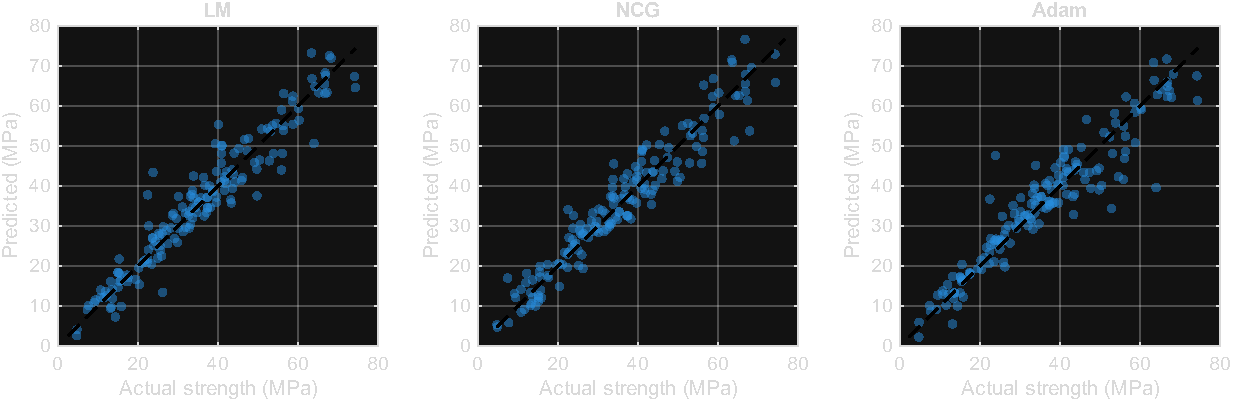
\includegraphics[width=\linewidth]{figures/pred_vs_actual.pdf}
\caption{Predicted vs.\ actual compressive strength on the test set
(MPa), seed 0. The line $y=x$ is shown for reference. Left: LM; middle:
NCG; right: Adam.}
\label{fig:pred-vs-actual}
\end{figure}
 
\subsection{Diagnostics}
\label{sec:res-diagnostics}
 
\Cref{fig:lm-lambda} shows the LM damping trajectory $\lambda_k$ for a
representative seed, illustrating the transition from near-steepest-descent
behavior (large $\lambda$) in the initial iterations toward
Gauss--Newton-like behavior (small $\lambda$) as the iterates approach a
minimizer. \Cref{fig:grad-norm} plots
$\norm{\grad L(\theta_k)}_\infty$ for all three methods; these curves are
useful for checking whether each method's empirical rate is qualitatively
consistent with its theoretical rate.
 
\begin{figure}[H]
\centering
\begin{subfigure}{0.48\linewidth}
  \centering
  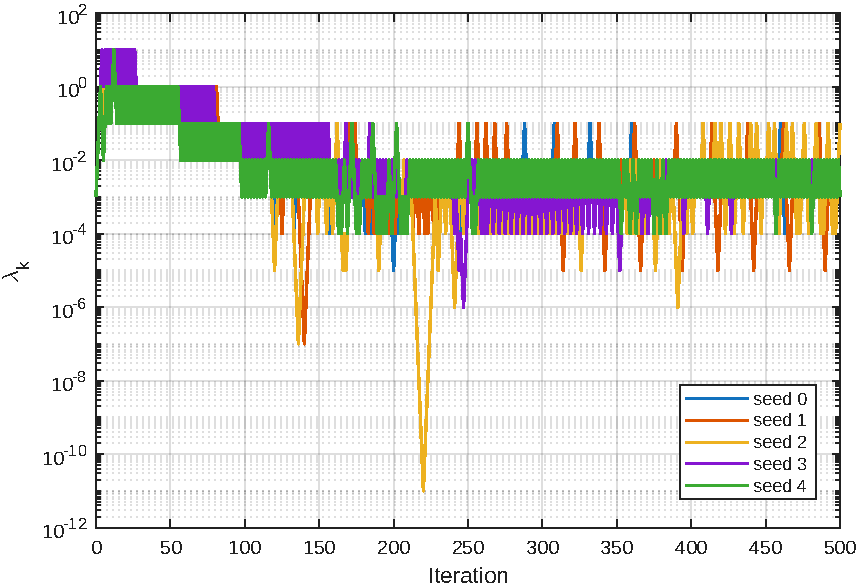
\includegraphics[width=\linewidth]{figures/lm_lambda.pdf}
  \caption{LM damping $\lambda_k$ vs.\ iteration.}
  \label{fig:lm-lambda}
\end{subfigure}\hfill
\begin{subfigure}{0.48\linewidth}
  \centering
  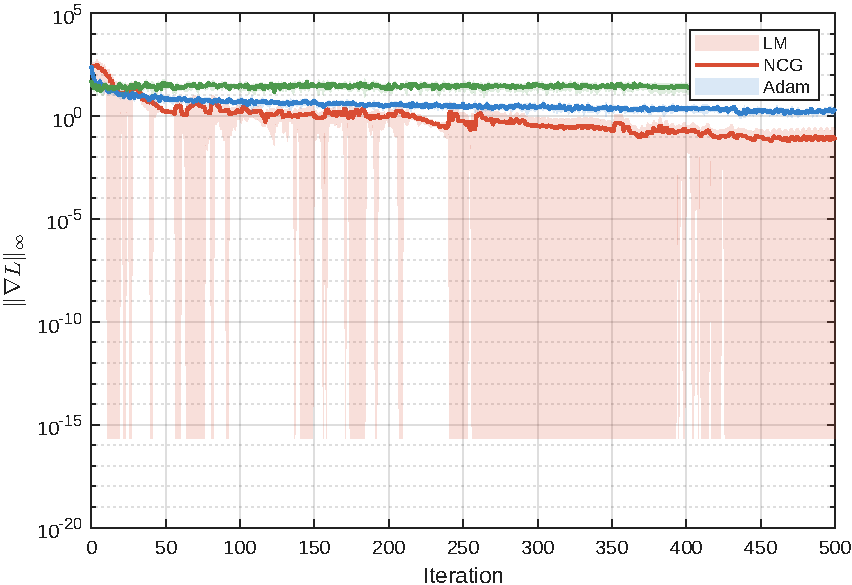
\includegraphics[width=\linewidth]{figures/grad_norm.pdf}
  \caption{$\norm{\grad L(\theta_k)}_\infty$ vs.\ iteration (log).}
  \label{fig:grad-norm}
\end{subfigure}
\caption{Optimizer diagnostics across the five seeds.}
\end{figure}
 
\subsection{Seed-to-seed variability}
 
\Cref{tab:seed-spread} reports final test RMSE for each method across the
five seeds individually, exposing robustness (or lack thereof) to
initialization.
 
\begin{table}[H]
\centering
\small
\caption{Test RMSE (MPa) by seed. Last column: spread (max $-$ min).}
\label{tab:seed-spread}
\begin{tabular}{@{}lrrrrrr@{}}
\toprule
Method & Seed 0 & Seed 1 & Seed 2 & Seed 3 & Seed 4 & Spread \\
\midrule
LM   & \texttt{[X]} & \texttt{[X]} & \texttt{[X]} & \texttt{[X]} & \texttt{[X]} & \texttt{[X]} \\
NCG  & \texttt{[X]} & \texttt{[X]} & \texttt{[X]} & \texttt{[X]} & \texttt{[X]} & \texttt{[X]} \\
Adam & \texttt{[X]} & \texttt{[X]} & \texttt{[X]} & \texttt{[X]} & \texttt{[X]} & \texttt{[X]} \\
\bottomrule
\end{tabular}
\end{table}
 
\subsection{Discussion of results}
\label{sec:discussion}
 
\paragraph{Does curvature information pay off?}
\texttt{[Paragraph summarizing whether LM's use of $J\T J$ yielded a
measurable advantage over NCG (no curvature) and Adam (diagonal
second-moment heuristic), with numbers from
\cref{tab:iters-to-tol,tab:time-to-tol,tab:test-rmse}. Interpret in light
of the problem scale $n = 305$.]}
 
\paragraph{Where does each method fail?}
\texttt{[Paragraph noting concrete failure modes observed: LM stagnation
when $J\T J$ is rank-deficient; NCG sensitivity to Wolfe line-search
failures and benefit of restarts; Adam instability at high learning rates.
Reference specific seeds or iteration ranges.]}
 
\paragraph{Methodological caveats.}
As noted in~\cref{rem:batch-asymmetry}, Adam is trained in mini-batch mode
while LM and NCG are full-batch. \texttt{[One or two sentences interpreting
how this asymmetry plausibly affects the comparison.]}
 
% =============================================================================
\section{Conclusions and recommendations}
\label{sec:conclusions}
% =============================================================================
 
\subsection{Summary of findings}
 
\texttt{[Three to five sentences summarizing what was done and what was
found. For example: ``We compared LM, NCG, and Adam on a neural-network
regression task framed as nonlinear least squares using the UCI Concrete
Compressive Strength dataset. Across five random seeds, \emph{method X}
achieved the lowest test RMSE (\texttt{[value $\pm$ std]} MPa),
\emph{method Y} was fastest in wall-clock time (\texttt{[value]} s), and
\emph{method Z} required the fewest iterations to reach the convergence
tolerance (\texttt{[value]}). These results [confirm / partially confirm /
contradict] the expectation that second-order information is advantageous
on small-to-medium-scale regression problems.'']}
 
\subsection{Method-specific takeaways}
 
\paragraph{Levenberg--Marquardt.}
\texttt{[One paragraph: on which axis (iterations / final loss /
wall-clock) did LM dominate; how did the damping trajectory behave; what
was the principal limitation observed.]}
 
\paragraph{Nonlinear Conjugate Gradient.}
\texttt{[One paragraph: NCG's placement on each axis; frequency of Wolfe
line-search failures (if any); whether Polak--Ribière\textsuperscript{+}
and restart schedule were sufficient to prevent cycling.]}
 
\paragraph{Adam.}
\texttt{[One paragraph: Adam's placement on each axis; best learning rate
found; sensitivity to that choice; whether mini-batch noise appeared
helpful or harmful for generalization.]}
 
\subsection{Answering the central question}
 
\texttt{[One paragraph answering: does curvature information pay off for
this problem class? Quantitative, with numbers from the results tables.
Include a projection of how the crossover would shift with problem scale,
consistent with the $O(n^3)$ cost of the LM linear solve.]}
 
\subsection{Limitations}
 
\begin{itemize}
  \item Single dataset; results may not generalize to other regression
    problems or to higher-dimensional feature spaces.
  \item Full-batch vs.\ mini-batch asymmetry between LM/NCG and Adam
    (\cref{rem:batch-asymmetry}) prevents a fully apples-to-apples
    comparison.
  \item The network architecture was fixed rather than jointly tuned per
    method; a method's performance partly reflects its interaction with
    this specific parametrization.
  \item Wall-clock comparisons are hardware- and implementation-dependent;
    MATLAB's internal \texttt{mldivide} benefits from optimized LAPACK
    routines that our NCG and Adam implementations do not exploit.
  \item The Gauss--Newton approximation~\cref{eq:gauss-newton} degrades in
    the large-residual regime, which is not systematically probed here.
\end{itemize}
 
\subsection{Recommendations}
 
\paragraph{For practitioners.}
\texttt{[Two or three actionable recommendations grounded in the findings.
For example: ``When the parameter count is below approximately
\texttt{[threshold]} and full-batch training is feasible, LM is
competitive with Adam on final accuracy and may converge in substantially
fewer iterations. For larger problems or online training, Adam remains
preferable. NCG rarely dominates but rarely disappoints, making it a
reasonable default when memory is constrained.'']}
 
\paragraph{For future work.}
\begin{enumerate}
  \item Extend the comparison to larger networks and datasets, to locate
    empirically the crossover point at which LM's per-iteration cost
    outweighs its convergence advantage.
  \item Investigate stochastic variants of LM (subsampled Gauss--Newton)
    to address the full-batch limitation.
  \item Include L-BFGS \citep[Ch.~6]{NocedalWright2006}, which occupies an
    intermediate point in the curvature-information spectrum and was
    omitted here for scope.
  \item Examine regimes in which the small-residual assumption underlying
    Gauss--Newton is violated, to characterize where LM loses its
    advantage.
\end{enumerate}
 
% =============================================================================
% References
% =============================================================================
\bibliographystyle{plainnat}
\bibliography{references}
 
\end{document}